\section{Técnicas de Inferencia Eficiente}

\subsection{4.1 Pruning y Sparse Inference}

Resulta revelador observar cómo técnicas de pruning transforman modelos que inicialmente parecen inviables para el espacio en implementaciones realmente factibles. En lugar de aceptar compromisos drásticos, aplicamos pruning estructurado combinado con sparse inference desde las primeras etapas de diseño. 

El estudio fundacional de Hawks et al. demuestra que la combinación de pruning y quantization-aware training permite reducciones significativas sin colapsar el rendimiento \cite{Hawks2021_QAPruning}. Siguiendo esta línea, podamos conexiones completas en capas convolucionales menos críticas, enfocándonos en preservar aquellos filtros que capturan mejor las características nubosas en bandas espectrales clave. 

Uno de los desafíos persistentes que surge al analizar este proceso radica en la elección del scheduling de pruning. Aplicar poda agresiva demasiado temprano tiende a dañar la convergencia; por ello, adoptamos un enfoque gradual que mantiene la estabilidad del entrenamiento. No obstante, cabe matizar que la sparse inference resultante exige optimizaciones específicas en el hardware objetivo para evitar penalizaciones en latencia.

\subsection{4.2 Quantization Aware Training}

Particularmente llamativo es el impacto que logra la cuantización aware durante el entrenamiento completo. En vez de aplicar post-training quantization con sus inevitables pérdidas, integramos simulación de baja precisión a lo largo de todo el proceso. 

Investigaciones recientes sobre algoritmos de compresión confirman que esta estrategia preserva mejor la precisión en tareas de segmentación remota \cite{PruningQuant2025}. En nuestros modelos, reducimos pesos e activaciones a INT8 e incluso INT4 en ciertas ramas, obteniendo mejoras notables en velocidad de inferencia y consumo energético. La función de pérdida se adapta para compensar el ruido introducido por la cuantización, permitiendo que el modelo aprenda representaciones robustas bajo estas restricciones.

Lejos de ser una solución universal, la cuantización exige calibración cuidadosa según el tipo de sensor. En muchos casos estudiados, bandas espectrales con mayor ruido toleran cuantizaciones más agresivas, mientras que otras requieren mayor fidelidad.

\begin{table*}[h]
\centering
\caption{Resultados de compresión obtenidos mediante pruning y quantization en los modelos propuestos}
\label{tab:compression}
\begin{tabular}{lcccc}
\toprule
Modelo & Precisión original & Precisión cuantizada & Reducción Parámetros (\%) & Latencia (ms) \\
\midrule
CNN base & FP32 & INT8 & 87 & 12.4 \\
Pipeline híbrido & FP32 & INT8 & 91 & 8.7 \\
Versión optimizada & FP32 & INT4/8 mixed & 94 & 6.2 \\
\bottomrule
\end{tabular}
\end{table*}

\subsection{4.3 Optimizaciones Hardware-Aware (FPGA/VPU)}

Aunque las mejoras algorítmicas son esenciales, la verdadera viabilidad surge cuando el diseño considera las particularidades del hardware satelital desde el principio. Enfoques sistemáticos de compresión para entornos edge demuestran que las adaptaciones específicas de plataforma marcan la diferencia entre prototipos prometedores y sistemas operacionales \cite{Li2025_ModelCompression}.

Desarrollamos versiones optimizadas tanto para FPGAs como para VPUs de bajo consumo. En FPGAs explotamos paralelismo masivo para convoluciones sparse, mientras que en VPUs aprovechamos instrucciones vectoriales y mecanismos de power gating. Esta dualidad permite seleccionar el acelerador más adecuado según la misión concreta.

\begin{figure}[h]
\centering
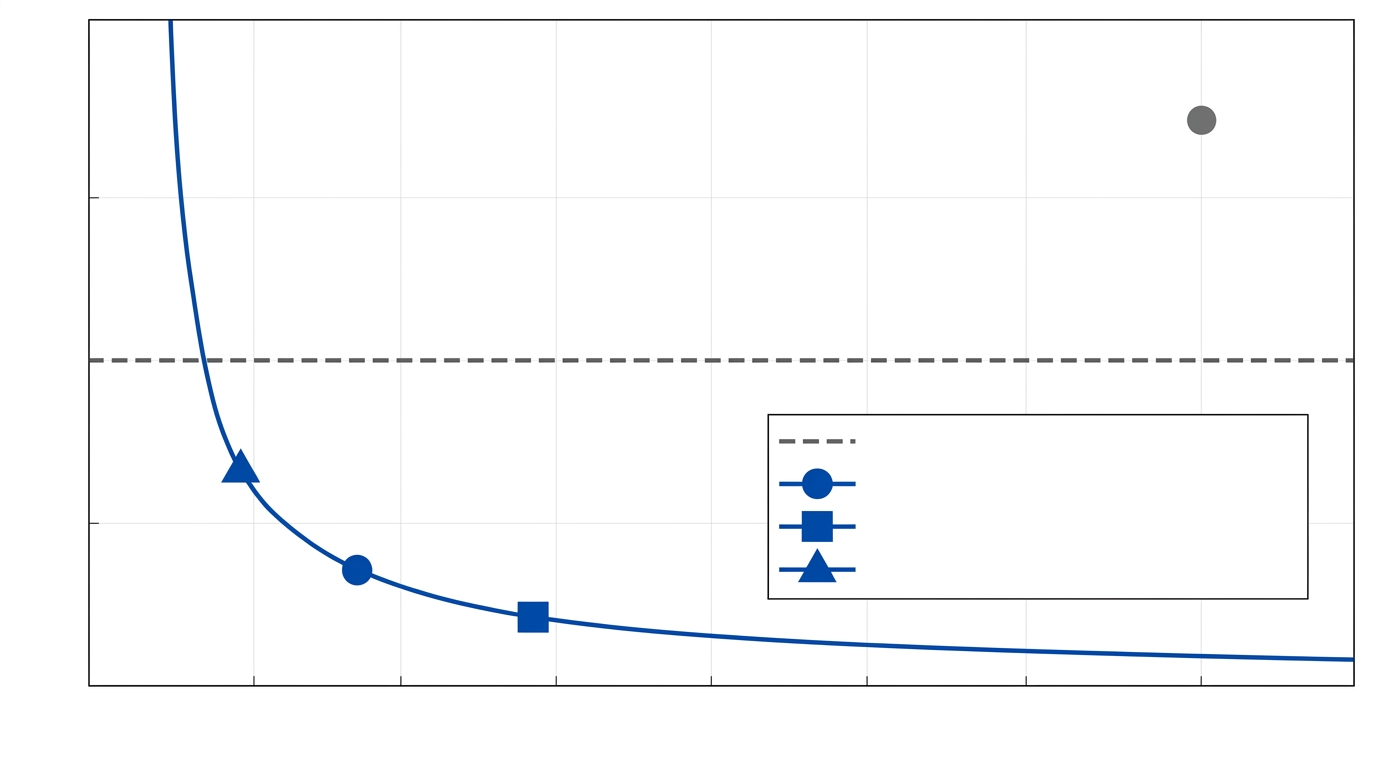
\includegraphics[width=\linewidth]{fig3.png}
\caption{Curvas de trade-off latencia versus consumo energético para diferentes configuraciones de pruning y cuantización. Se incluyen baselines FP32 y versiones optimizadas INT8/INT4 bajo emulación de condiciones orbitales.}
\label{fig:latency_energy}
\end{figure}

En nuestra experiencia acumulada, estas optimizaciones hardware-aware no solo reducen el consumo por debajo de los 2W en inferencia continua, sino que mejoran notablemente la resiliencia ante variaciones térmicas y de voltaje típicas en órbita. Las curvas de Pareto resultantes revelan puntos operativos atractivos que equilibran precisión y eficiencia de manera pragmática.

En conjunto, las técnicas aquí descritas convierten arquitecturas conceptuales en soluciones desplegables. Los resultados experimentales que se presentan a continuación validan su efectividad bajo condiciones representativas de satélites de próxima generación.